% Collaboration patterns — stop-at-first-match decision tree.
% Author from scratch (no source LaTeX analog). Same yes/no decision-tree
% shape that Ch 8's extension-decision will use, for visual consistency.
\documentclass[tikz,border=4mm]{standalone}
\usepackage{tikz}
\usetikzlibrary{positioning, shapes.geometric, arrows.meta, calc}

\begin{document}
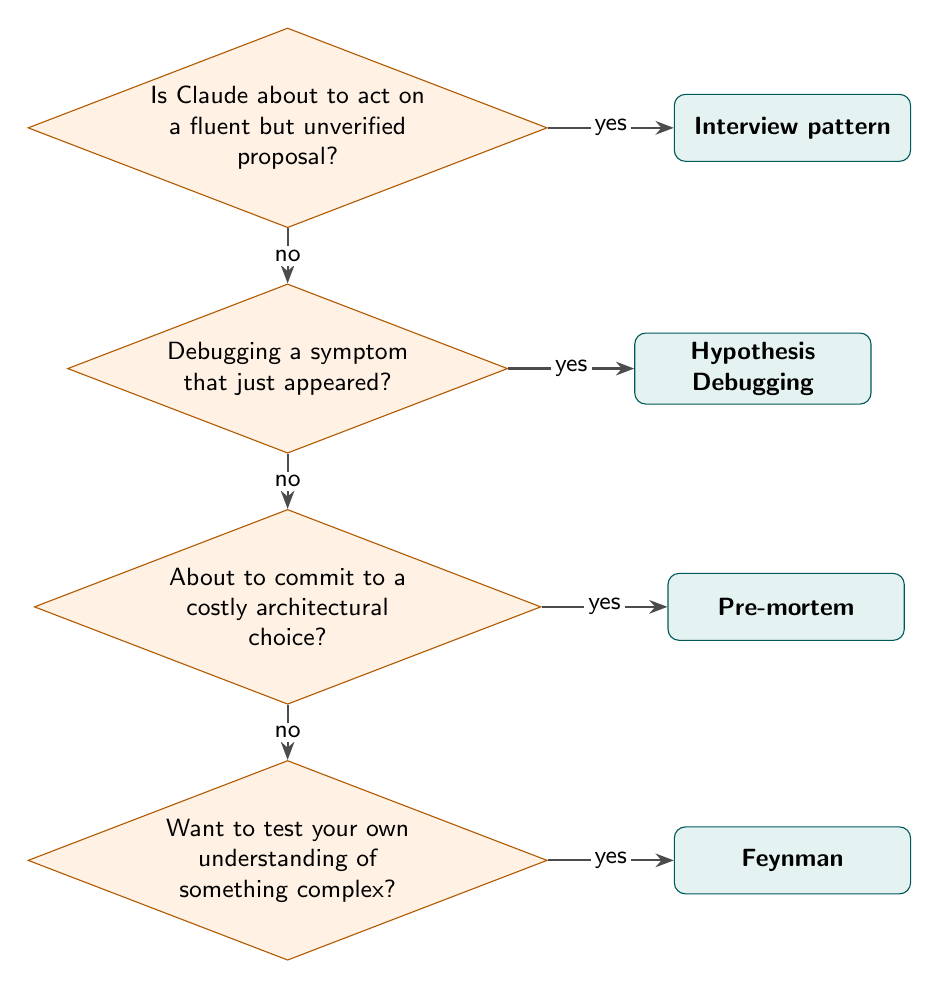
\begin{tikzpicture}[
  font=\sffamily,
  node distance=0.7cm and 1.6cm,
  question/.style={
    draw=orange!70!black, fill=orange!10, diamond, aspect=2.6,
    inner sep=1pt, align=center, text width=3.6cm, font=\sffamily\small
  },
  pattern/.style={
    draw=teal!70!black, fill=teal!10, rounded corners=4pt,
    minimum width=3cm, minimum height=0.85cm, align=center,
    font=\sffamily\small\bfseries
  },
  arrow/.style={-Stealth, thick, draw=gray!60!black},
  arrowlabel/.style={font=\sffamily\small, fill=white, inner sep=1.5pt},
]

% Decision chain (top → bottom) with patterns to the right
\node[question] (q1) {Is Claude about to act on \\ a fluent but unverified \\ proposal?};
\node[pattern, right=of q1] (interview) {Interview pattern};

\node[question, below=of q1] (q2) {Debugging a symptom \\ that just appeared?};
\node[pattern, right=of q2] (hyp) {Hypothesis \\ Debugging};

\node[question, below=of q2] (q3) {About to commit to a \\ costly architectural \\ choice?};
\node[pattern, right=of q3] (pre) {Pre-mortem};

\node[question, below=of q3] (q4) {Want to test your own \\ understanding of \\ something complex?};
\node[pattern, right=of q4] (feynman) {Feynman};

% Arrows: yes goes right; no goes down to next question
\draw[arrow] (q1) -- node[arrowlabel] {yes} (interview);
\draw[arrow] (q1) -- node[arrowlabel] {no} (q2);
\draw[arrow] (q2) -- node[arrowlabel] {yes} (hyp);
\draw[arrow] (q2) -- node[arrowlabel] {no} (q3);
\draw[arrow] (q3) -- node[arrowlabel] {yes} (pre);
\draw[arrow] (q3) -- node[arrowlabel] {no} (q4);
\draw[arrow] (q4) -- node[arrowlabel] {yes} (feynman);

\end{tikzpicture}
\end{document}
